\documentclass[a4paper,14pt]{extarticle} 
\usepackage[a4paper,top=1.5cm, bottom=1.5cm, left=2cm, right=1cm]{geometry}
%\usepackage[T2A]{fontenc}
%\usepackage[english, russian]{babel}
\usepackage{graphicx}
\DeclareGraphicsExtensions{.pdf,.png,.jpg}

\usepackage{fontspec}
\setmainfont{Times New Roman}
\setsansfont{FreeSans}
\setmonofont{FreeMono}
\renewcommand{\baselinestretch}{1.5}
\usepackage{polyglossia}
\setdefaultlanguage{russian}
\setotherlanguages{english,russian}
\usepackage{setspace}
\usepackage[many]{tcolorbox}

\begin{document}

    \begin{center}
        \thispagestyle{empty}
        \begin{singlespace}
        ФЕДЕРАЛЬНОЕ АГЕНТСТВО СВЯЗИ

        ФЕДЕРАЛЬНОЕ ГОСУДАРСТВЕННОЕ БЮДЖЕТНОЕ ОБРАЗОВАТЕЛЬНОЕ

        УЧРЕЖДЕНИЕ ВЫСШЕГО ОБРАЗОВАНИЯ

        «САНКТ-ПЕТЕРБУРГСКИЙ ГОСУДАРСТВЕННЫЙ УНИВЕРСИТЕТ ТЕЛЕКОММУНИКАЦИЙ ИМ. ПРОФ. М.А. БОНЧ-БРУЕВИЧА»

        (СПбГУТ)
        \end{singlespace}
        \vspace{-1ex}
        \rule{\textwidth}{0.4pt}
        \vspace{-5ex}

        Факультет \underline{Инфокоммуникационных сетей и систем}

        Кафедра \underline{Защищенных систем связи}
        \vspace{10ex}

        \textbf{Лабораторная работа №1}

    \end{center}
    \vspace{4ex}
    \begin{flushright}
    \parbox{8cm}{
    \begin{flushleft}
        Выполнил:

        \underline{Громов А.А., ИКТЗ-83} \hfill \rule[-0.85ex]{0.1\textwidth}{0.6pt}

        \footnotesize \textit{ (Ф.И.О., № группы) \hfill (подпись)} \normalsize

        Проверил:

        \underline{Гельфанд А.М.} \hfill \rule[-0.85ex]{0.1\textwidth}{0.6pt}

        (\footnotesize \textit{уч. степень, уч. звание, Ф.И.О.) \hfill (подпись)} \normalsize

    \end{flushleft}
    }
    \end{flushright}
    \begin{center}
        \vfill
        Санкт-Петербург

        2020

        \end{center}

    \newpage
    \begin{center}
        \textbf{\large{ Введение}}
    \end{center}

    Цель работы:\\ 
    1) Создать коммутатор, маршрутизатор, компьютер.\\
    2) Соединить их в сеть.\\ 
    3) Задать на коммутаторе и маршрутизаторе пароль, зашифрованный и 
    незашифрованный соотвтетственно.\\
    4) Настроить на компьютере и на порте роутера ip адреса из одной 
    локальной сети.\\
    
    Топология сети:
    \begin{center}
        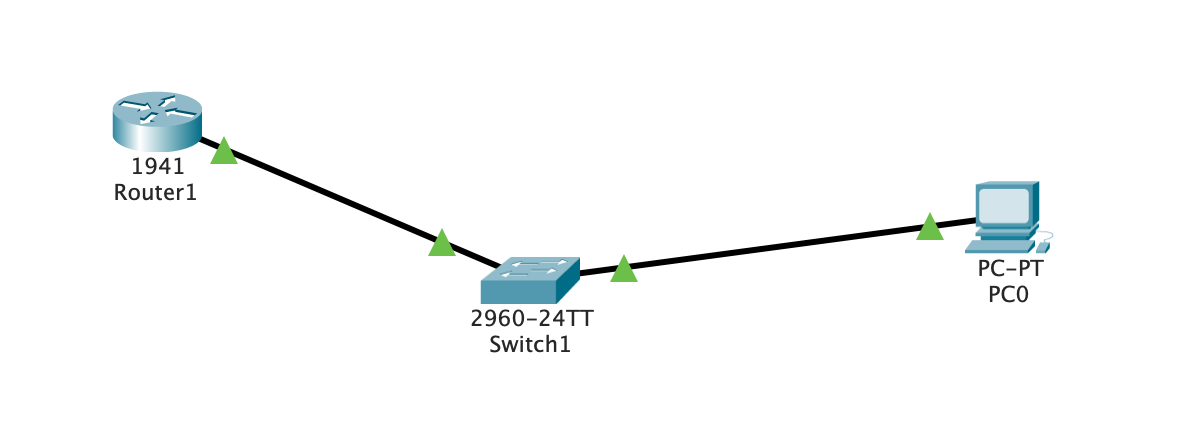
\includegraphics[scale=0.7]{net.png}
    \end{center}

    Команды на Роутере:\\
    - en\\
    - conf t\\
    - ho R1\\
    - enable password cisco\\
    - int gi0/0\\
    - ip address 192.168.0.1 255.255.255.0\\
    - no shutdown\\
    - end\\
    - sh run\\
    
    log:
    \begin{singlespace}
        \begin{tcolorbox}
            Building configuration...\\
            Current configuration : 646 bytes\\
            !\\
            version 15.1\\
            no service timestamps log datetime msec\\
            no service timestamps debug datetime msec\\
            no service password-encryption\\
            !\\
            hostname R1\\
            !\\
            enable password cisco\\
            !\\
            no ip cef\\
            no ipv6 cef\\
            !\\
            license udi pid CISCO1941/K9 sn FTX15244SSW-\\
            !\\
            spanning-tree mode pvst\\
            !\\
            interface GigabitEthernet0/0\\
            ip address 192.168.0.1 255.255.255.0\\
            duplex auto\\
            speed auto\\
            !\\
            interface GigabitEthernet0/1\\
            no ip address\\
            duplex auto\\
            speed auto\\
            shutdown\\
            !\\
            interface Vlan1\\
            no ip address\\
            shutdown\\
            !\\
            ip classless\\
            !\\
            ip flow-export version 9\\
            !\\
            line con 0\\
            !\\
            line aux 0\\
            !\\
            line vty 0 4\\
            login\\
            !\\
            end
        \end{tcolorbox} 
    \end{singlespace}
    Команды на Коммутаторе: \\
    - en\\
    - conf t\\
    - enable secret cisco\\
    - service password-encryption\\ 
    - end\\
    - sh run\\

    log:
    \begin{singlespace}
        \begin{tcolorbox}[breakable]
            Building configuration...\\
            Current configuration : 1157 bytes\\
            !\\
            version 12.2\\
            no service timestamps log datetime msec\\
            no service timestamps debug datetime msec\\
            service password-encryption\\
            !\\
            hostname S1\\
            !\\
            enable secret 5 \$1\$mERr\$hx5rVt7rPNoS4wqbXKX7m0\\
            !\\
            spanning-tree mode pvst\\
            spanning-tree extend system-id\\
            !\\
            interface FastEthernet0/1\\
            !\\
            interface FastEthernet0/2\\
            !\\
            interface FastEthernet0/3\\
            !\\
            interface FastEthernet0/4\\
            !\\
            interface FastEthernet0/5\\
            !\\
            interface FastEthernet0/6\\
            !\\
            interface FastEthernet0/7\\
            !\\
            interface FastEthernet0/8\\
            !\\
            interface FastEthernet0/9\\
            !\\
            interface FastEthernet0/10\\
            !\\
            interface FastEthernet0/11\\
            !\\
            interface FastEthernet0/12\\
            !\\
            interface FastEthernet0/13\\
            !\\
            interface FastEthernet0/14\\
            !\\
            interface FastEthernet0/15\\
            !\\
            interface FastEthernet0/16\\
            !\\
            interface FastEthernet0/17\\
            !\\
            interface FastEthernet0/18\\
            !\\
            interface FastEthernet0/19\\
            !\\
            interface FastEthernet0/20\\
            !\\
            interface FastEthernet0/21\\
            !\\
            interface FastEthernet0/22\\
            !\\
            interface FastEthernet0/23\\
            !\\
            interface FastEthernet0/24\\
            !\\
            interface GigabitEthernet0/1\\
            !\\
            interface GigabitEthernet0/2\\
             shutdown\\
            !\\
            interface Vlan1\\
             no ip address\\
             shutdown\\
            !\\
            line con 0\\
             password 7 0822455D0A16\\
            !\\
            line vty 0 4\\
             login\\
            line vty 5 15\\
             login\\
            !\\
            end
        \end{tcolorbox}
    \end{singlespace}

    Выдаем нашему ПК адрес 192.168.0.2 с маской 255.255.255.0 
    и шлюзом 192.168.0.1\\

    Проверяем связь:\\
    Заходим на маршрутизатор и прописываем команду ping:\\
    - ping 192.168.0.2\\
    log:
    \begin{singlespace}
        \begin{tcolorbox}
            Type escape sequence to abort.\\
            Sending 5, 100-byte ICMP Echos to 192.168.0.2, timeout is 2 seconds:\\
            .!!!!\\
            Success rate is 80 percent (4/5), round-trip min/avg/max = 0/0/0 ms
        \end{tcolorbox}
    \end{singlespace}
     



\end{document}